\documentclass[margin=10pt]{standalone}
\usepackage{amsmath}
\usepackage{pgfplots}
\pgfplotsset{compat=1.3}

\newcommand\clipright[1][white]{
  \fill[#1](current axis.south east)rectangle(current axis.north-|current axis.outer east);
  \pgfresetboundingbox
  \useasboundingbox(current axis.outer south west)rectangle([xshift=.5ex]current axis.outer north-|current axis.east);
}

\definecolor{mycolor}{rgb}{0.02,0.4,0.7}

\begin{document}
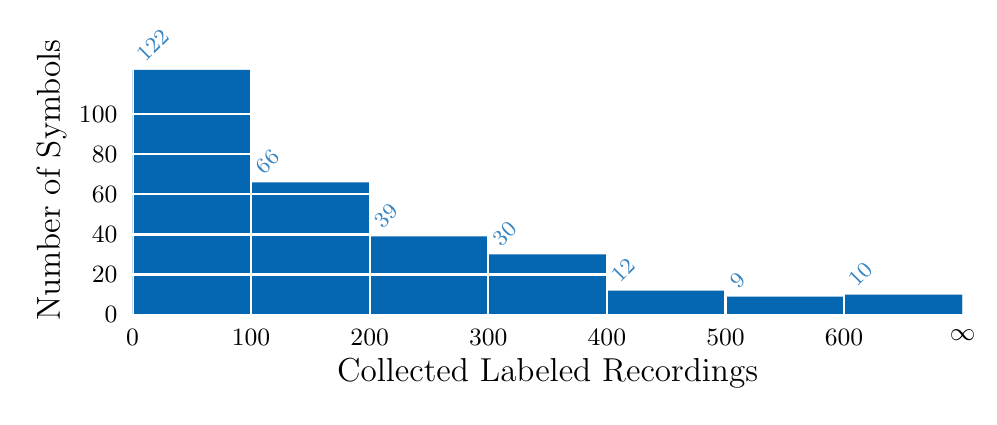
\begin{tikzpicture}
    \begin{axis}[
        ymajorgrids,
        xmajorgrids,
        grid style={white,thick},
        axis on top,
        /tikz/ybar interval,
        tick align=outside,
        ymin=0,
        axis line style={draw opacity=0},
        tick style={draw=none},
        enlarge x limits=false,
        height=5cm,
        title style={font=\Large},
        xlabel={Collected Labeled Recordings},
        ylabel={Number of Symbols},
        ytick={ 0,20,40,60,80,100 },
        scaled ticks=false,
        yticklabels={ 0, 20, 40, 60, 80, 100 },
        xticklabels={ $0$, $100$, $200$, $300$, $400$, $500$, $600$, $\infty$ },
        width=\textwidth,
        xtick=data,
        label style={font=\large},
        ticklabel style={
            inner sep=1pt,
            font=\small
        },
        nodes near coords,
        every node near coord/.append style={
            fill=white,
            anchor=mid west,
            shift={(3pt,4pt)},
            inner sep=0,
            font=\footnotesize,
            rotate=45},
            ]
    \addplot[mycolor!80!white, fill=mycolor, draw=none] coordinates { (0, 122) (1, 66) (2, 39) (3, 30) (4, 12) (5, 9) (6, 10) (7, 70)  };
    \end{axis}
    \clipright
\end{tikzpicture}
\end{document}